
\chapter{Bibliographic revision}



%\chapter{Justiça em aprendizado de máquina}
%\section{Justiça, transparência, auditabilidade e privacidade}
%\section{Fontes de injustiça}
%section{Definições e métricas}
%\section{Regulamentação}
%\section{Conjuntos de dados}
%\section{Abordagens para classificação justa}
%\section{Otimização multiobjetivo}

%\chapter{Ruído em aprendizado de máquina}
%\section{Definições e taxonomia de ruído}
%\section{Classificação na presença de ruído de classe}
%\section{Fatoração e correção de funções de custo}
%\section{Estimadores da matriz de transição}



In this section, we review pertinent literature on fair machine learning, placing a particular emphasis on in-processing techniques. We also delve into classification methodologies that operate in the presence of label noise and discuss multi-objective optimization within the context of fair machine learning. While our research does not directly tackle fairness problems in the presence of label noise, we highlight relevant works that, akin to ours, bridge the domains of fairness and noise in machine learning research. 

\subsection{Fair Classification}

In this paper, we focus on some of the most widely used fairness definitions in classification problems, as described by \cite{Verma2018} and summarized by \cite{Mehrabi2019} and \cite{caton2023}. These definitions include demographic parity, equal opportunity, predictive equality, and equalized odds.

It's crucial to understand that no single fairness definition universally applies to all scenarios. The choice of a particular fairness definition and metric should be informed by ethical considerations grounded in the social context in which the model would be deployed~\citep{AlerTubella2022}. Selecting a fairness definition is not a purely technical matter, as it inevitably entails ethical and social considerations that should not be neglected. Building fair machine learning models requires an interdisciplinary approach that engages all stakeholders, including specially those who are typically marginalized or underrepresented~\citep{Weinberg2022}.  Here we describe some frequently used definitions and metrics.

\begin{definition}[Statistical Parity]\label{def:demo_parity}
The likelihood of a positive, i.e. favorable, outcome should be the same in every group of the sensitive attribute~\citep{Dwork2011,Kusner2018}. A binary predictor $\hat{Y}$ satisfies Statistical Parity (a.k.a. Demographic Parity) if $P(\hat{Y}|A=0) = P(\hat{Y}|A=1)$, where $A$ is a protected attribute.
\end{definition}

Demographic Parity does not depend on true class $Y$, only on prediction $\hat{Y}$. We can measure Demographic Parity (Definition~\ref{def:demo_parity}) for a protected attribute $A$ as the absolute difference between $P(\hat{Y}|A=0)$ and $P(\hat{Y}|A=1)$. According Demographic Parity, the predictor is considered fairer when this metric is lower. 

\begin{definition}[Equal Opportunity]\label{def:eq_opp}
The probability of a person in a positive class being assigned to a positive, i.e. favorable, outcome should be the same in every group of the sensitive attribute~\citep{Hardt2016}. A binary predictor $\hat{Y}$ satisfies Equal Opportunity if $P(\hat{Y}|A=0,Y=1) = P(\hat{Y}|A=1,Y=1)$, where $Y$ is true class and $A$ is a protected attribute.
\end{definition}

Definition~\ref{def:eq_opp} claims that protected and unprotected, i.e. privileged, groups should have equal true positive rates. Mathematically, a classifier with equal true positive rates will also have equal false negative rates. Like in Demographic Parity, we can measure Equal Opportunity as an absolute difference between protected and privileged group rates. A variation of Equal Opportunity is Predictive Equality (Definition~\ref{def:pred_eq}).

\begin{definition}[Predictive Equality]\label{def:pred_eq}
The probability of a person in a negative class being assigned to a negative outcome should be the same in every group of the sensitive attribute. A binary predictor $\hat{Y}$ satisfies Predictive Equality if $P(\hat{Y}|A=0,Y=0) = P(\hat{Y}|A=1,Y=0)$, where $Y$ is true class and $A$ is a protected attribute.
\end{definition}

Equalized Odds is a combination of the principles from Definition~\ref{def:eq_opp} and Definition~\ref{def:pred_eq}, i.e., protected and unprotected groups should have equal true positive and true negative rates, therefore equal false positive and false negative rates. We can measure Equalized Odds as the average between Equal Opportunity and Predictive Equality.

\begin{definition}[Equalized Odds]\label{def:eq_odds}
Both probabilities of the person in a positive class being assigned to a positive outcome and of a person in a negative class being assigned to a negative outcome should be the same in every group of the sensitive attribute~\citep{Hardt2016}. A binary predictor $\hat{Y}$ satisfies Equalized Odds (a.k.a. Average Odds Difference) if $P(\hat{Y}|A=0,Y) = P(\hat{Y}|A=1,Y)$, where $Y$ is true class and $A$ is a protected attribute.
\end{definition}

Fairness intervention methods can be classified into three categories based on the stage at which they occur, as proposed by \cite{Mehrabi2019} and \cite{AlerTubella2022}: Pre-processing methods intervene before learning, modifying the data to reduce existing biases; In-processing methods intervene during learning by modifying the objective functions or imposing constraints to the model in order to mitigate discriminatory effects; Post-processing methods affects predictions produced by the model after learning to change possibly unfair outcomes. In this work, we incorporate information about disparities among social groups in the dataset into our model by modifying the loss function through the use of a transition matrix. This fairness intervention is thus classified as an in-processing technique.

Other relevant in-processing strategies for fair classification include Naive Bayes approaches for discrimination-free classification~\citep{Calders2010}, Fairness Through Awareness Framework~\citep{Dwork2011}, Fairness-Aware Classifier with Prejudice Remover Regularizer~\cite{Kamishima2012}, $\alpha$-discriminatory empirical risk minimizer~\citep{Woodworth2017}, Disparate Impact and Disparate Mistreatment frameworks for margin-based classifiers~\citep{Zafar2017a,Zafar2017b}, Weak Agnostic Learning to Auditing Subgroup Fairness~\citep{pmlr-v80-kearns18a,Kearns2018}, One-Network Adversarial Fairness~\citep{Adel2019}, FairGan$^{+}$ ~\citep{Xu2019}, Monte Carlo policy gradient method~\citep{Petrovic2021}, Fairness-accuracy Pareto~\citep{Wei2022}, and Pareto front stochastic multi-gradient~\citep{Liu2022} based in original stochastic multi-gradient~\citep{Mercier2018} to Multi-Objective Optimization and the hybrid Adaptive Priority Reweighing approach~\cite{HuXT23}.

Recently, special attention has been given in fair machine learning research topics like addressing multiple sensitive attributes or multiple classes \cite{DAloisio2023,Liu_Wang_Wang_Wang_Su_Gao_2023}, loss balancing techniques~\cite{KIM2023231,KhaliliZA23}, where the objective is to balance the loss across different groups instead of predictive metrics, adversarial approaches~\cite{Liang2023,ZhangZLZY23,GrariLD23,MousaviMD23,Zeming2023,Yuchen2023} and the privacy concerns involving fairness under federated learning settings~\cite{ChenZZZY24,VucinichZ23}. Another relevant research topic in fair machine learning is learning under censored data~\cite{WZhang2022,WZhang2023_a,WZhang2023_b,WZhang2023_c}, which we will discuss in section~\ref{sec:fairness_noise}.

\subsection{Multi-Objective Optimization}

A model that substantially decreases model performance to reduce unfairness may not be a viable option, as low performance could harm all groups affected by the model's decisions, including protected groups. Similarly, a model projected to be a fair alternative that keeps performance almost intact, but with little or even no gain in fairness, is not practically relevant. It is possible that fine-tuning this trade-off could result in a fairer solution that achieves better performance than traditional methods, but this is not the case for most practical problems. Achieving this balance is one of the most challenging tasks in fair machine learning.

In this context, an interesting approach is to deal with fair machine learning as a Multi-Objective Optimization (MOO) problem, where predictive performance and fairness metric are the objectives, which could be defined according Equation~\ref{def:moo}, where $\lambda$ is a parameter configuration in the space $\Lambda$, $\rho: \Lambda \mapsto [0,1]$ is a model performance metric and $\varphi: \Lambda \mapsto [0,1]$ a fairness metric. The set of all optimal solutions is called Pareto front, where one objective cannot be improved without sacrificing another. In this setting there is no single $\lambda^*$ optimal solution, but a set of solutions forming a Pareto front~\citep{pareto1906manuale}.

\begin{align}\label{def:moo}
\max &\hspace{1ex} (\rho(\lambda), \varphi(\lambda)) \\
\text{subject to} &\hspace{1ex} \lambda\in\Lambda \nonumber
\end{align}

One of the most frequent approach to deal with MOO problems like these is to combine the multiple function outputs to a single scalar, which is called scalarization. Therefore, we could describe a general scalarization setup to Equation~\ref{def:moo} according Equation~\ref{def:scalarized_moo}. The effectiveness of this approach is that is also possible to use single objective optimization techniques to tackle the MOO optimization problem. In this scenario a relevant issue is to select a scalarization setup capable of promote a proper trade-off of all the objectives thorough the optimization process given the optimization method.

\begin{equation}\label{def:scalarized_moo}
\arg\max\limits_{\lambda\in\Lambda} G(\lambda) = (\rho(\lambda), \varphi(\lambda))
\end{equation}

The fairness-accuracy Pareto front is formally described in \cite{Wei2022}, which demonstrate that many existing fairness methods are performing a linear scalarization scheme and argues that it has several limitations in recovering Pareto optimal solutions. Instead, authors proposes a Chebyshev scalarization scheme, that is theoretically superior than linear scheme. A characterization of the accuracy-fairness trade-off as a Pareto front can be found in \cite{Liu2022}. Also, \cite{Mercier2018} proposes a stochastic multi-gradient based in original stochastic multi-gradient to Multi-Objective Optimization.

Another remarkable use of MOO in Fair Machine Learning is to perform a Fair Hyperparameter Optimization, which can offer a model agnostic approach with flexibility to apply in multiple machine learning pipelines. A time-efficient Baysian Optimization approach can be found in \cite{Schmucker2020}, combining scalarization techniques with the bandit-inspired Hyperband \citep{Li2016} algorithm to Hyperparameter Optimization in context of fairness.

A general objective function to be used with some popular off-the-shelf hyperparameters optimization techniques combining model performance and fairness in a flexible setting can be found in \cite{Cruz2021}. The authors argues that in fairness context the Pareto front is most often convex, thus proposes a simple scalarizing function that could be applied to reduce $G$ to a single scalar with weighed $l_p$-norm. Also, they argue that \cite{GIAGKIOZIS2015338} demonstrate the the  use  of $l_p$-norms with a high $p$ value leads to slower convergence. Thus, the optimization metric $g(\lambda) = ||G(\lambda)||_1$ is optimized according Equation~\ref{eq:moo_smoothed_2}, where $\alpha$ is the relative importance of predictive performance and fairness and $\lambda$ is a parameter configuration in the space $\Lambda$. In experiments, $\alpha$ is fixed at $0.5$, giving same importance to both objectives.

\begin{equation} \label{eq:moo_smoothed_2}
    G(\lambda) = \alpha \cdot \rho(\lambda) + (1-\alpha) \cdot \varphi(\lambda)
\end{equation}

A Multi-objective SVMOptimizer with Dataset Constraints is proposed by \cite{Goh2016}, where the objective is to minimize multiple objectives on real-world datasets, such as misclassification error and positive prediction at specific rate to some population. A custom reinforcement learning algorithm directly modeling performance and fairness as objectives is proposed by \cite{Petrovic2021}. Authors proposes using as reward function the difference between model performance (Area Under the ROC Curve) and three different fairness metrics (Statistical Parity, Equal Opportunity and Equalized Odds), each one with its respective importance coefficient. In experimental setups only one of those coefficient are different from zero. Thus, the optimized metric could be written as $G(\lambda) = \rho(\lambda) - \alpha \cdot \varphi(\lambda)$, where $\alpha$ is the relative importance of fairness.

\subsection{Classification in the presence of label noise}

The presence of noise in data can substantially decrease model performance in classification problems. Noise can be defined as non systematic errors that obscures the relationship between features of an instance and its class~\citep{Frenay2014,Hickey1996,Quinlan1986}. Two types of noise are found in literature, in features (or attributes) and in labels (or classes). Feature noise affects observed values, e.g. by adding a small Gaussian noise on each feature during measurement. Likewise, label noise change the observed label assigned to an instance, e.g. by randomly inverting labels in a binary classification problem. Although feature noise could affect model performance, label noise is potentially more harmful, since we frequently have many features and only one label. Note that in label noise only the observed label of an instance is affected, its true class remains the same.

The label noise taxonomy considers three types of noise: Noisy Completely at Random, Noisy at Random, and Noisy Not at Random~\citep{Frenay2014}. Figure~\ref{fig:taxonomia} presents the statistical dependency between features $X$, class $Y$, observed label $\tilde{Y}$ and the occurrence of error E, i.e. $E=1$ when $Y \neq \tilde{Y}$. The simplest type is Noisy Completely at Random, where the occurrence of error $E$ not depend on $X$ and $Y$, e.g. randomly flipping labels on a binary classification problem. In Noisy at Random, the occurrence of error $E$ depends only on $Y$, e.g. randomly flipping labels on binary classification with different rates for positives and negatives classes. Noisy Not at Random considers the occurrence of error $E$ depending on both $Y$ and $X$, e.g. flipping labels on binary classification with different rates for each group of instances of a certain feature.


 \begin{figure}[!htb]
 \centering
\caption{Noise taxonomy from a statistical perspective. (a) completely random noise (NCAR), (b) random noise (NAR) and (c) non-random noise (NNAR). The arrows correspond to the statistical dependencies. For clarity, the dependency between $X$ and $Y$ was placed as a dashed arrow.}
 \label{fig:taxonomia}
 \scalebox{1.0}{%
    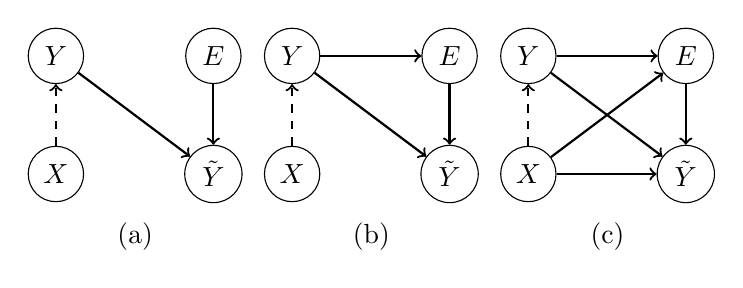
\begin{tikzpicture}[main_node/.style={circle,draw,minimum size=2em,inner sep=3pt]}]

     \node[main_node] (1) at (-1, 0) {$Y$};
     \node[main_node] (2) at (-1, -1.5)  {$X$};
     \node[main_node] (3) at (1, -1.5) {$\tilde{Y}$};
     \node[main_node] (4) at (1, 0) {$E$};
     \path[->,draw,thick]
     (1) edge node {} (3)
     (4) edge node {} (3)
     ;
    
     \path[->,dashed,thick]
     (2) edge node {} (1)
     ;
    
     \node[below=2cm] at (current bounding box.base) {(a)};
    
     \begin{scope}[xshift=3cm,grow=right,baseline]
     
     \node[main_node] (1) at (-1, 0) {$Y$};
     \node[main_node] (2) at (-1, -1.5)  {$X$};
     \node[main_node] (3) at (1, -1.5) {$\tilde{Y}$};
     \node[main_node] (4) at (1, 0) {$E$};

     \path[->,draw,thick]
     (1) edge node {} (3)
     (4) edge node {} (3)
     (1) edge node {} (4)
     ;
    
     \path[->,dashed,thick]
     (2) edge node {} (1)
     ;
    
     \node[below=2cm,xshift=1.5cm] at (current bounding box.base) {(b)};
    
     \end{scope}
    
     \begin{scope}[xshift=6cm,grow=right,baseline]
     \node[main_node] (1) at (-1, 0) {$Y$};
     \node[main_node] (2) at (-1, -1.5)  {$X$};
     \node[main_node] (3) at (1, -1.5) {$\tilde{Y}$};
     \node[main_node] (4) at (1, 0) {$E$};

     \path[->, draw,thick]
     (1) edge node {} (3)
     (4) edge node {} (3)
     (1) edge node {} (4)
     (2) edge node {} (3)
     (2) edge node {} (4)
     ;
    
     \path[->,dashed,thick]
     (2) edge node {} (1)
     ;
    
     \node[below=2cm,xshift=3cm] at (current bounding box.base) {(c)};
    
     \end{scope}
 \end{tikzpicture}
 }
 \end{figure}

Many label noise robustness methods can be found on literature, in this work we highlight the \textit{backward} and \textit{forward} loss corrections, proposed by \cite{Patrini2017} using concepts of loss factorization~\citep{Patrini2016}. Those loss correction techniques considers a NAR label noise, which is described by a transition matrix $T$ such as 
\begin{equation}
    T_{i,j} = P(\tilde{Y} = y_j|Y = y_i),
\end{equation}
where $\mathcal{Y} = \{y_1, y_2, \ldots, y_c\}$ is the set of all possible class labels. Transition matrix includes corruption probabilities for every possible label combination, each value represents the probability of one label be corrupted onto another. This matrix is row-stochastic and not necessarily symmetric across the classes.
\begin{equation} \label{eq:backward}
    \ell^{\leftarrow}(P(\tilde{Y}|X)) = T^{-1} \ell(P(\tilde{Y}|X))
\end{equation}

The backward loss correction is defined by Equation~\ref{eq:backward} to an arbitrary loss function $\ell$ and a transition matrix $T$. The backward loss correction involves a linear combination of the loss values for each observed label, using coefficients that depends on the probability that each observed label reflects the true class. Intuitively, we are reweighting the loss according to the noise probabilities of each label using the inverse of T and thus somehow going one step back, reverting the noise effects. This corrected loss is unbiased and can be minimized with any conventional back-propagation algorithm, making it flexible to include within different training techniques and data pipelines.
\begin{equation} \label{eq:forward}
    \ell^{\rightarrow}(P(\tilde{Y}|X)) = \ell(T^{\top} P(\tilde{Y}|X))
\end{equation}

However, backward correction requires matrix inversion, which may not exist or may lead to numerical instabilities if the transition matrix T is ill-conditioned. Although there is possible solutions to a bad condition number of T, one should consider using the forward correction, a backward variation proposed by \cite{Patrini2017} to avoid this issue, as defined in Equation~\ref{eq:forward}. While backward acts on the loss itself, forward corrects model predictions. Forward correction does not have the same theoretical guarantees as backward, but offers a label noise robustness, ensuring that the learned model is the minimize over the clean distribution without the need of matrix inversion.

\subsection{Fairness in the presence of noise}\label{sec:fairness_noise}

Some recent works deal with fairness problems in the presence of noise. For example, the sensitive attribute available could be noisy, which could distort the effects of fairness intervention. In this context, \cite{Lamy2019} uses noise-rate estimators from the label noise literature to change a fairness model. Also, \cite{Fogliato2020} proposes a framework for assessing how assumptions on the noise across groups affect the predictive bias properties in risk assessment models. Furthermore, \cite{Wang2020} considers the consequences of naively relying on noisy protected group labels while proposing two new optimization approaches with sensitive attribute noise robustness. A denoised version of the selection problem to deal with noisy sensitive attributes is proposed in \cite{Mehrotra2021}. Lastly, \cite{Celis2021} proposes an optimization framework for classification in the presence of noisy protected attributes.

There is also the perspective of dealing with the proxy features divergence or covariance. A theoretical approach to this issue identifying potential sources of errors can be found in \cite{Prost2021}. The problem of measuring group fairness in ranking based on divergence with proxy features is investigated by \cite{Ghazimatin2022}. A framework of fair semi-supervised learning in the pre-processing phase can be found in \cite{Zhang2022}, which includes predicting labels for unlabeled data, a resampling method, and ensemble learning to improve accuracy and decrease discrimination.

Another research direction is considering how fair models perform in the presence of NNAR label noise, where error rates of corruption depend both on the label class and the membership of a protected subgroup. In this scenario \cite{Wang2021} addresses the problem of fair classification and \cite{Wu2022} provides a general framework for rewriting the classification risk and the fairness metric in terms of noisy data and thereby building robust classifiers. In \cite{Ghosh2023} a study about the presence of noise in the protected attribute can be found.

Furthermore, many recent works deals with fairness under semi-supervised settings considering censored data, that is, for some individuals the class label is not available due censorship~\cite{WZhang2022,WZhang2023_a,WZhang2023_b,WZhang2023_c}. In this scenario, the main approach is to use some technique to estimate the missing data instead of removing the instance from training data. This is closely related to the previous problems of fair learning under noisy data. In censored fairness problems noise can be interpreted as a kind of censorship, as the original data affected by noise is not available.

Bias and noise are two related phenomena, both corrupt data affecting models trained with this data. For example, if noise disproportionately affects different groups this potentially produces unfairness in models that uses this data in training~\citep{Wang2021}. For example, we could have positive true class ($Y = 1$) flipped into negative labels ($\tilde{Y} =0$) more frequently in the protected group ($A = 1$) than in privileged group ($A = 0$). Simultaneously, the negative class ($Y = 0$) could be more frequently flipped into positives observed labels ($\tilde{Y} = 1$) within privileged/unprotected group ($A = 0$). This scenario could lead to a undetected higher false negative rate to protected group and higher false positive rate to privileged group. In this case the Noisy Not at Random data would be a source of negative social bias.

In \cite{Mehrabi2019} a non-exhaustive list of bias types was presented, including \textit{Historical Bias}, \textit{Representation Bias}, \textit{Sampling Bias}, \textit{Omitted Variable Bias}, among others. In the scenario described above, the incorrect measurement of the true class resulted in a different observed label ($Y \neq \tilde{Y}$), which could be classified as a \textit{Measurement Bias}. Similarly, a Noisy Not at Random data could lead to a \textit{Population Bias}, where the characteristics of the population represented in the data differ from those of the original target population.

It can be challenging to distinguish between label noise and bias in certain scenarios, specially when noise disproportionately affects different social groups. Although there is some overlapping, they are distinct phenomena. Label noise is a stochastic process that is considered independent and unintentional~\citep{Frenay2014}, whereas bias is rooted in historical and social issues and could be intentional. Furthermore, even noise-free data, correctly represented by observed features and labels, may be unfair since the social phenomena that produce this data could be biased against some groups. %Thus, the objective of this work is not to theoretically deal with fair machine learning as a label noise problem or incorporate noisy classes or attributes in fairness problems. 

Prior studies in the realm of fairness have largely concentrated on understanding how noisy or censored data affects fair learning and on mitigating these effects. In contrast, our approach is inspired by label noise techniques, but with a distinct goal: not merely to analyze or mitigate the impact of noise or censorship, but to directly address and reduce unfairness itself.